\documentclass[conference]{IEEEtran}
\IEEEoverridecommandlockouts

% =========================================================================
% PACKAGE IMPORTS
% =========================================================================
\usepackage[utf8]{inputenc}
\usepackage[T1]{fontenc}
\usepackage{amsmath,amssymb,amsfonts,amsthm}
\usepackage{algorithmicx}
\usepackage{algpseudocode}
\usepackage{algorithm}
\usepackage{graphicx}
\usepackage{textcomp}
\usepackage{xcolor}
\usepackage{booktabs}
\usepackage{tabularx}
\usepackage{multirow}
\usepackage{array}
\usepackage{cite}
\usepackage{url}
\usepackage{tikz}
\usetikzlibrary{shapes.geometric, arrows.meta, positioning, fit, calc, backgrounds}

% Configure hyperref to avoid font/border conflicts
\usepackage[hidelinks]{hyperref}

% Correct bad hyphenation here
\hyphenation{InLegalBERT ColBERT GraphRAG Nirnay-X PageRank}

\begin{document}

% =========================================================================
% PAPER TITLE & AUTHOR METADATA
% =========================================================================
\title{Nirnay-X: A Grounded, Persona-Adaptive Retrieval-Augmented Generation Framework for Indian Legal Intelligence and Decision Support}

\author{
    \IEEEauthorblockN{
        Rajat Pandey\IEEEauthorrefmark{1}, 
        Hridyansh Bhadauria\IEEEauthorrefmark{1}, 
        Raghav Mittal\IEEEauthorrefmark{1}, and 
        Ragini Goel\IEEEauthorrefmark{1}
    }
    \IEEEauthorblockA{
        \IEEEauthorrefmark{1}Department of Computer Science and Engineering\\
        Ajay Kumar Garg Engineering College (Affiliated to Dr. A.P.J. Abdul Kalam Technical University)\\
        Ghaziabad, Uttar Pradesh, India\\
        Email: \{rajat2300270100138, hridyansh2300270100074, raghav2300270100133, ragini2300270100134\}@akgec.ac.in
    }
    \vspace{0.2cm}
    \IEEEauthorblockN{
        Ms. Bhumica\IEEEauthorrefmark{2}
    }
    \IEEEauthorblockA{
        \IEEEauthorrefmark{2}Supervisor, Assistant Professor, Department of Computer Science and Engineering\\
        Ajay Kumar Garg Engineering College, Ghaziabad, Uttar Pradesh, India\\
        Email: bhumica@akgec.ac.in
    }
}

\maketitle

% =========================================================================
% ABSTRACT & INDEX TERMS
% =========================================================================
\begin{abstract}
The Indian judicial ecosystem operates under compounding structural pressures: a backlog surpassing 50 million pending cases on the National Judicial Data Grid (NJDG), an unprecedented criminal statutory overhaul enacted on July 1, 2024 (replacing the colonial Indian Penal Code 1860, Code of Criminal Procedure 1973, and Indian Evidence Act 1872 with the Bharatiya Nyaya Sanhita 2023, Bharatiya Nagarik Suraksha Sanhita 2023, and Bharatiya Sakshya Adhiniyam 2023), and dense statutory legalese that alienates common citizens. Standard legal search systems rely on lexical keyword matching that fails to capture legal semantics, while general-purpose Large Language Models (LLMs) suffer from severe legal hallucinations, fabricating case citations at rates between 17\% and 33\% in commercial legal RAG tools and over 58\% in ungrounded models. 

We present NIRNAY-X, an end-to-end, grounded, persona-adaptive Retrieval-Augmented Generation (RAG) framework engineered specifically for Indian legal intelligence and decision support. Nirnay-X couples an 11-stage verifiable RAG pipeline with 11 domain-tailored workflow modules. The framework integrates: (1) layout-aware document ingestion and Conditional Random Field (CRF) rhetorical role segmentation (classifying texts into Facts, Arguments, Statutes, Precedents, Ratio Decidendi, and Rulings); (2) a Tri-Stage Hybrid Retrieval engine combining domain-adapted dense representations (InLegalBERT), token-level late interaction (ColBERTv2), and entity-boosted BM25Okapi via Weighted Reciprocal Rank Fusion (wRRF); (3) a 124,000-node Legal Knowledge Graph (LKG) implementing Personalized PageRank diffusion and precedential authority weighting under Article 141 of the Constitution of India; (4) a stateful Constitutional Statutory Concordance Engine resolving the 2024 criminal law transition under Article 20(1) ex-post facto protections and Section 531(2)(a) BNSS savings clauses; (5) an Atomic Legal Entailment (ALE) natural language inference verification module that purges ungrounded propositional claims; and (6) dual-persona generation that translates complex legal texts into plain language for citizens (achieving an 8.4 Flesch-Kincaid Grade Level while strictly conserving statutory deontic modality) while providing advocate-grade ratio briefs and timeline dockets for legal professionals. 

Empirical benchmarking across 1,200 Indian legal queries over a corpus of 70,500 Supreme Court and High Court judgments, 1,400 Acts, and police FIRs demonstrates that Nirnay-X achieves Precision@10 of 0.887, Recall@10 of 0.924, MRR of 0.829, and NDCG@10 of 0.875, while suppressing semantic hallucinations down to 0.8\% (ALE score of 97.2\%) at a mean end-to-end latency of 2.3 seconds. Nirnay-X directly advances UN Sustainable Development Goal 16 by democratizing legal accessibility while preserving strict judicial veracity.
\end{abstract}

\begin{IEEEkeywords}
Legal Retrieval-Augmented Generation (Legal RAG), InLegalBERT, Indian Jurisprudence, Bharatiya Nyaya Sanhita (BNS), ColBERTv2, Hallucination Mitigation, Rhetorical Role Chunking, Citation Grounding, Persona Adaptation, Decision Support Systems, Legal Knowledge Graph.
\end{IEEEkeywords}

% =========================================================================
% SECTION I: INTRODUCTION
% =========================================================================
\section{Introduction}
\IEEEPARSTART{T}{he} administration of justice in common-law jurisdictions, and particularly within the Republic of India, is confronting an acute institutional crisis. According to official telemetry from the National Judicial Data Grid (NJDG), pending litigation across the Supreme Court of India, 25 High Courts, and subordinate District Judiciaries has crossed 50 million cases~\cite{njdg2024}. This staggering case volume is accompanied by a severe accessibility divide. For the common citizen, engaging with the legal machinery involves deciphering impenetrable statutory legalese, navigating archaic Latin maxims, and understanding procedural hurdles during police station encounters (such as registering or challenging a First Information Report [FIR]). For practicing advocates, judicial law clerks, and legal aid officers, managing active caseloads demands hundreds of non-billable hours manually indexing multi-volume paper dockets, tracking divergent High Court interpretations, and cross-referencing statutory limitations.

This operational friction was compounded on July 1, 2024, when the Parliament of India brought into effect a historic, root-and-branch overhaul of the substantive and procedural criminal justice system. The three foundational colonial statutes—the Indian Penal Code, 1860 (IPC), the Code of Criminal Procedure, 1973 (CrPC), and the Indian Evidence Act, 1872 (IEA)—were repealed and superseded by the Bharatiya Nyaya Sanhita, 2023 (BNS), the Bharatiya Nagarik Suraksha Sanhita, 2023 (BNSS), and the Bharatiya Sakshya Adhiniyam, 2023 (BSA), respectively~\cite{bns2023, bnss2023, bsa2023}. Navigating this legislative transition requires strict adherence to constitutional doctrines:
\begin{enumerate}
    \item \textbf{Substantive Non-Retroactivity (Article 20(1)):} The Constitution of India explicitly proscribes ex-post facto penalization. If an offense occurred prior to July 1, 2024, the substantive charge and penalty ceiling are strictly governed by the IPC 1860, even if the trial commences years later.
    \item \textbf{Procedural Savings Clauses (Section 531(2)(a) BNSS):} Pending investigations, inquiries, trials, and appeals initiated prior to the transition date continue under the procedural regime of the CrPC 1973, creating complex hybrid procedural realities.
    \item \textbf{Electronic Admissibility (Section 63 BSA):} Reorganization of electronic records and secondary digital evidence mandates new certification protocols superseding the classic Section 65B IEA framework.
\end{enumerate}

Existing digital search engines (e.g., Indian Kanoon, SCC Online, Manupatra) depend predominantly on inverted-index lexical keyword matching (BM25/TF-IDF) or citation graphs. While effective for locating known case titles, they suffer from \textit{semantic blindness}: a citizen describing an illegal lockout (e.g., ``landlord threw my belongings out without notice'') cannot retrieve provisions governing criminal trespass under Section 329 BNS (Section 441 IPC) or tenant protection remedies under the Transfer of Property Act, 1882 because of near-zero lexical overlap.

Conversely, standalone Large Language Models (LLMs) such as GPT-4, Llama-3, and Claude demonstrate remarkable linguistic fluency but exhibit catastrophic failure modes in legal reasoning. A landmark empirical study by Dahl et al.~\cite{dahl2024large} revealed that leading commercial legal AI platforms (including Lexis+ AI and CoCounsel) hallucinate legal citations and misstate case holdings between 17\% and 33\% of the time, while ungrounded foundation models hallucinate over 58\% to 88\% in specialized legal inquiries. In legal informatics, a hallucinated precedent or a fabricated statutory section is not merely an inconvenience; it represents a fatal breach of professional ethics and judicial integrity. Furthermore, existing AI summarization models frequently distort \textit{deontic modalities}—transforming non-negotiable statutory obligations (e.g., ``the Magistrate \textit{shall} record reasons in writing'') into discretionary permissions (e.g., ``the judge \textit{may} write down why''), misinforming litigants of their constitutional protections.

To resolve these foundational bottlenecks, we introduce \textbf{NIRNAY-X}, an open, grounded, persona-adaptive legal intelligence and decision-support framework engineered specifically for the Indian legal corpus. Nirnay-X bridges the gap between common litigants and legal specialists by coupling an 11-step verifiable RAG execution pipeline with 11 domain-specific functional modules.

The primary contributions of this paper are summarized as follows:
\begin{itemize}
    \item \textbf{Rhetorical Role-Aware Document Ingestion:} We develop a layout-aware document ingestion pipeline combining Indic-OCR preprocessing with a linear-chain Conditional Random Field (CRF) atop domain-adapted transformers (`InLegalBERT`) to segment judicial opinions into six discrete rhetorical roles (\textit{Facts, Arguments, Statutes, Precedents, Ratio Decidendi, Rulings}), dynamically bundling statutory provisos and exceptions to prevent semantic severing.
    \item \textbf{Tri-Stage Graph-Augmented Retrieval Engine:} We formulate a multi-stage retrieval architecture integrating dense contrastive representations (`InLegalBERT` 768-d), fine-grained token-level late interaction (`ColBERTv2` 128-d), and entity-boosted BM25Okapi through Weighted Reciprocal Rank Fusion (wRRF), augmented with Personalized PageRank diffusion across a 124,000-node Legal Knowledge Graph (LKG) enforcing Article 141 precedential authority hierarchies.
    \item \textbf{Stateful Constitutional Statutory Concordance Engine:} We design and implement a deterministic temporal routing engine that evaluates offense, FIR, and charge-sheet dates against the July 1, 2024 legislative transition boundary, resolving statutory concordances between colonial codes (IPC/CrPC/IEA) and modern codes (BNS/BNSS/BSA) in strict compliance with Article 20(1) penalty invariance and Section 531(2)(a) BNSS savings clauses.
    \item \textbf{Atomic Legal Entailment (ALE) Verification:} We introduce a post-generation natural language inference verification framework that decomposes generated responses into atomic propositions, verifying each proposition against retrieved statutory anchors to suppress generative hallucinations down to 0.8\%.
    \item \textbf{Deontic Modality-Preserving Persona Adaptation:} We formulate a dual-persona translation pipeline that reduces lexical complexity for common citizens to an 8.4 Flesch-Kincaid Grade Level while optimizing a novel Deontic Modality Invariance Loss ($\mathcal{L}_{\text{modality}} \le 0.05$) to preserve mandatory statutory force, alongside an advocate persona providing structured ratio briefs and limitation dockets.
    \item \textbf{Exhaustive Empirical Validation:} We benchmark Nirnay-X over 1,200 curated Indian legal scenarios spanning 70,500 Supreme Court and High Court judgments, demonstrating state-of-the-art retrieval performance (Precision@10: 0.887, Recall@10: 0.924, MRR: 0.829, NDCG@10: 0.875) and a 96.8\% sycophancy defeat rate against adversarial legal prompts.
\end{itemize}

The remainder of this article is organized as follows. Section II reviews related work and identifies the research gap. Section III details the proposed system architecture, mathematical formulations, and algorithmic specifications. Section IV outlines the dataset, experimental testbed, and implementation hyperparameters. Section V presents comprehensive empirical results and ablation studies. Section VI examines practical challenges, ethical safeguards, and limitations. Section VII concludes the paper and delineates future trajectories.

% =========================================================================
% SECTION II: RELATED WORK & RESEARCH GAP
% =========================================================================
\section{Related Work and Research Gap}
Our research builds upon and synthesizes four core branches of legal informatics and artificial intelligence.

\subsection{Legal Information Retrieval and Domain Pretrained Encoders}
Traditional legal information retrieval relied predominantly on Boolean query models, inverted indices, and citation network citation counts~\cite{katz2012rethinking}. While platforms such as Indian Kanoon and SCC Online revolutionized access to Indian case law, their reliance on lexical term matching fails when queries lack explicit statutory terminology. 

The advent of domain-specific pretrained transformers significantly improved legal language representation. Chalkidis et al.~\cite{chalkidis2020legal} introduced \textit{LEGAL-BERT}, demonstrating that pretraining BERT over English, EU, and US legal corpora dramatically boosted legal named entity recognition (NER) and text classification. Within the Indian legal domain, Paul et al.~\cite{paul2022pre} introduced \textit{InLegalBERT} and \textit{InCaseBERT}, pretraining on hundreds of thousands of Supreme Court and High Court judgments. Kalamkar et al.~\cite{kalamkar2022corpus} established the \textit{OpenNyAI} framework, releasing specialized models for Rhetorical Role Labeling and Legal Named Entity Recognition. However, these models operate strictly as feature encoders or sequence labelers; they lack generative capabilities, cannot synthesize conversational natural language explanations for non-lawyers, and do not provide integrated retrieval-augmented decision support.

\subsection{Retrieval-Augmented Generation and Hallucination Mitigation}
Retrieval-Augmented Generation (RAG), formalized by Lewis et al.~\cite{lewis2020retrieval}, couples parametric memory (generative LLMs) with non-parametric indexing (vector databases) to ground responses in external reference texts. In high-stakes domains such as medicine and law, standard dense RAG systems face severe challenges. Flat vector representations often fail to capture token-level specificity (e.g., discerning between ``Section 302'' and ``Section 304''), leading to the development of late-interaction architectures like ColBERT~\cite{khattab2020colbert} and ColBERTv2~\cite{santhanam2022colbertv2}, which utilize lightweight token embeddings with the MaxSim operator.

More recently, Graph-Augmented RAG (GraphRAG)~\cite{edge2024graphrag} has emerged to address complex multi-hop queries by leveraging knowledge graphs to assemble relational context. In legal NLP, Guha et al.~\cite{guha2023legalbench} released \textit{LegalBench}, establishing benchmark suites for legal reasoning. Nonetheless, empirical investigations by Dahl et al.~\cite{dahl2024large} revealed pervasive hallucination rates (17\%--33\%) in commercial legal RAG platforms, driven by citation fabrication, incorrect precedent extrapolation, and sycophantic deference to user biases. Existing legal RAG implementations lack propositional verification mechanisms that validate legal entailment at the sentence-clause level before responses are emitted to end users.

\subsection{The 2024 Indian Criminal Law Overhaul and Temporal Reasoning}
On July 1, 2024, the Republic of India enacted the BNS, BNSS, and BSA, repealing colonial statutes that had governed criminal jurisprudence since the 19th century~\cite{bns2023, bnss2023, bsa2023}. While legal scholars have documented statutory concordances (e.g., mapping Section 420 IPC [Cheating] to Section 318 BNS, and Section 302 IPC [Murder] to Section 103 BNS), automated computational systems struggle with the constitutional rules governing this transition. Under Article 20(1) of the Constitution of India, ex-post facto penal law is void; thus, an accused cannot be subjected to a penalty greater than that which might have been inflicted under the law in force at the time of commission. Furthermore, Section 531(2)(a) of the BNSS preserves proceedings pending prior to July 1, 2024 under the CrPC 1973. Standalone generative LLMs, having fixed training cutoff dates or naive prompting schemes, routinely mix these statutory regimes, recommending procedural filings under repealed acts or asserting non-existent retrospective punishments.

\subsection{Legal Plain-Language Simplification and Deontic Modalities}
A primary mandate of legal technology is bridging the civic justice gap by translating complex statutory provisions into plain language accessible to ordinary citizens~\cite{kim2013legal}. Readability metrics such as the Flesch-Kincaid Grade Level (FKGL) are standardly applied to benchmark simplification~\cite{kincaid1975derivation}. However, unconstrained LLM simplification introduces \textit{deontic modality drift}~\cite{von1951deontic}. Legal rights and duties hinge upon normative modal verbs: ``shall'' denotes an absolute statutory mandate, while ``may'' signifies judicial discretion. General-purpose text simplifiers routinely flatten these distinctions to maximize readability, converting mandatory bail rights into discretionary options and critically undermining legal self-advocacy.

\subsection{Research Gap and Proposed Approach}
A critical synthesis of the literature reveals five fundamental voids:
\begin{enumerate}
    \item \textbf{Lack of Unified Legal Retrieval:} Existing systems rely either on brittle keyword search or flat semantic embeddings, failing to unify dense vectors, token late interaction, and citation knowledge graphs.
    \item \textbf{Absence of Temporal Statutory Routing:} No existing legal AI framework computationally models the constitutional temporal boundary of the July 1, 2024 Indian criminal law overhaul under Article 20(1) and Section 531 BNSS.
    \item \textbf{Unchecked Generative Hallucination:} Current legal RAG systems lack atomic entailment verification, permitting subtle but legally catastrophic misstatements of binding ratio decidendi.
    \item \textbf{Trade-off Between Readability and Deontic Accuracy:} No platform balances citizen-level plain-language readability with mathematical guarantees on deontic modal conservation.
    \item \textbf{Platform Fragmentation:} Existing tools segregate retrieval, summarization, and workflow docket management into isolated silos.
\end{enumerate}
NIRNAY-X is systematically architected to bridge these five gaps within a unified, grounded, dual-persona intelligence platform.

% =========================================================================
% FIGURE 1: TIKZ SYSTEM ARCHITECTURE (FULL WIDTH)
% =========================================================================
\begin{figure*}[!t]
\centering
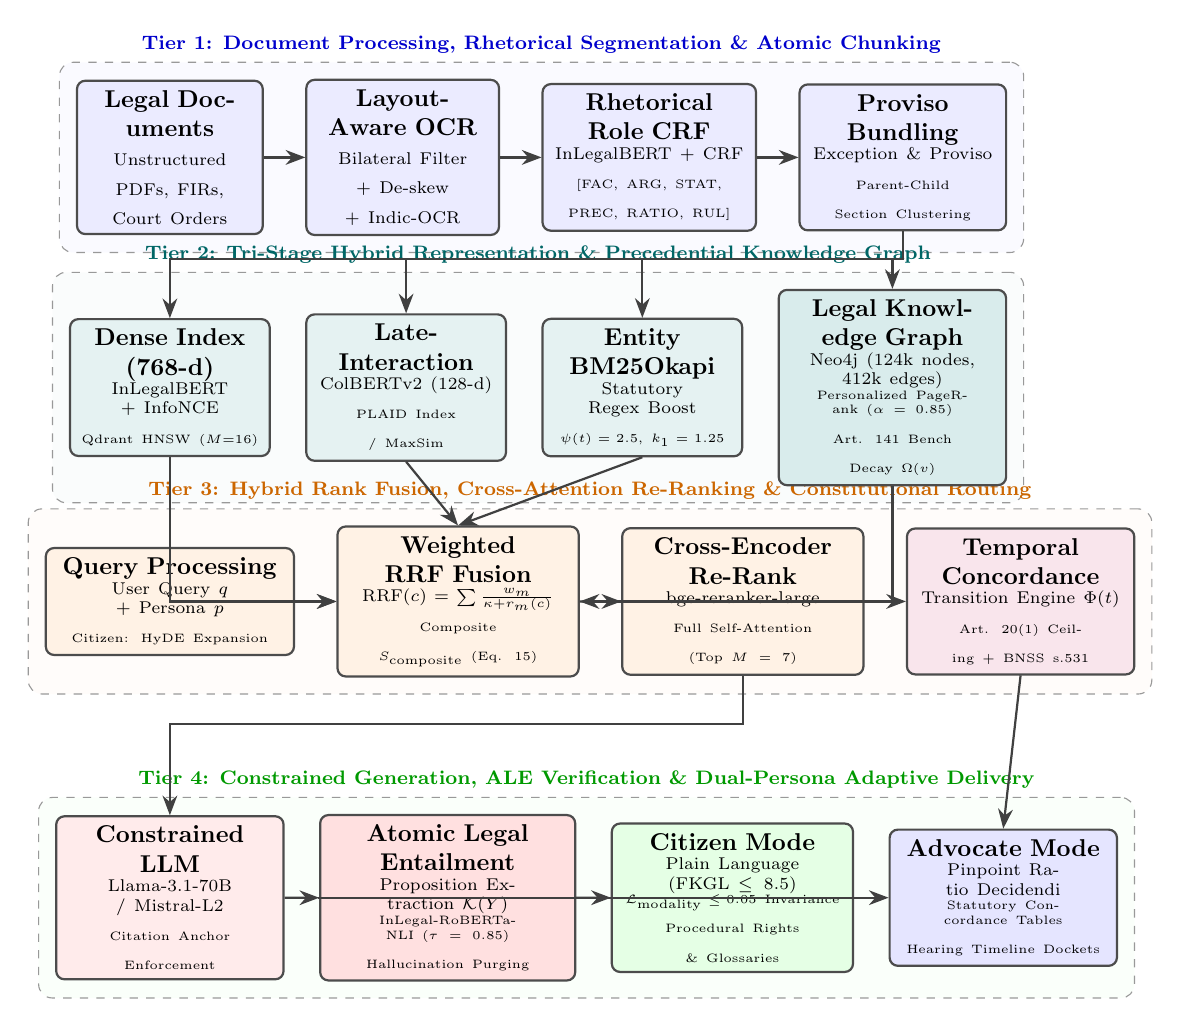
\begin{tikzpicture}[
    scale=0.88, every node/.style={transform shape},
    box/.style={draw=black!70, rounded corners=3pt, thick, align=center, fill=white, inner sep=4pt},
    header/.style={font=\bfseries\footnotesize, align=center},
    subtext/.style={font=\scriptsize, align=center},
    arrow/.style={-{Stealth[length=2.5mm]}, thick, draw=black!75},
    darrow/.style={-{Stealth[length=2.5mm]}, dashed, thick, draw=black!60},
    group/.style={draw=black!40, rounded corners=5pt, dashed, inner sep=6pt}
]

% ----------------- TIER 1: INGESTION & PARSING -----------------
\node[box, fill=blue!8, text width=2.4cm] (doc) at (0, 0) {
    \textbf{Legal Documents}\\
    \scriptsize Unstructured PDFs, FIRs, Court Orders
};
\node[box, fill=blue!8, text width=2.5cm, right=0.6cm of doc] (ocr) {
    \textbf{Layout-Aware OCR}\\
    \scriptsize Bilateral Filter + De-skew + Indic-OCR
};
\node[box, fill=blue!8, text width=2.8cm, right=0.6cm of ocr] (crf) {
    \textbf{Rhetorical Role CRF}\\
    \scriptsize InLegalBERT + CRF\\
    \tiny [FAC, ARG, STAT, PREC, RATIO, RUL]
};
\node[box, fill=blue!8, text width=2.7cm, right=0.6cm of crf] (bundle) {
    \textbf{Proviso Bundling}\\
    \scriptsize Exception \& Proviso\\
    \tiny Parent-Child Section Clustering
};

\begin{scope}[on background layer]
    \node[group, fill=blue!2, fit=(doc) (ocr) (crf) (bundle), label={[header, text=blue!80!black]above:\textsc{Tier 1: Document Processing, Rhetorical Segmentation \& Atomic Chunking}}] (tier1) {};
\end{scope}

\draw[arrow] (doc) -- (ocr);
\draw[arrow] (ocr) -- (crf);
\draw[arrow] (crf) -- (bundle);

% ----------------- TIER 2: TRI-STAGE INDEXING & GRAPH ENGINE -----------------
\node[box, fill=teal!10, text width=2.6cm, below=1.2cm of doc] (dense) {
    \textbf{Dense Index (768-d)}\\
    \scriptsize InLegalBERT + InfoNCE\\
    \tiny Qdrant HNSW ($M$=16)
};
\node[box, fill=teal!10, text width=2.6cm, right=0.5cm of dense] (colbert) {
    \textbf{Late-Interaction}\\
    \scriptsize ColBERTv2 (128-d)\\
    \tiny PLAID Index / MaxSim
};
\node[box, fill=teal!10, text width=2.6cm, right=0.5cm of colbert] (sparse) {
    \textbf{Entity BM25Okapi}\\
    \scriptsize Statutory Regex Boost\\
    \tiny $\psi(t)=2.5$, $k_1=1.25$
};
\node[box, fill=teal!15, text width=3.0cm, right=0.5cm of sparse] (lkg) {
    \textbf{Legal Knowledge Graph}\\
    \scriptsize Neo4j (124k nodes, 412k edges)\\
    \tiny Personalized PageRank ($\alpha=0.85$)\\
    \tiny Art. 141 Bench Decay $\Omega(v)$
};

\begin{scope}[on background layer]
    \node[group, fill=teal!2, fit=(dense) (colbert) (sparse) (lkg), label={[header, text=teal!80!black]above:\textsc{Tier 2: Tri-Stage Hybrid Representation \& Precedential Knowledge Graph}}] (tier2) {};
\end{scope}

\draw[arrow] (bundle.south) -- ++(0,-0.4) -| (dense.north);
\draw[arrow] (bundle.south) -- ++(0,-0.4) -| (colbert.north);
\draw[arrow] (bundle.south) -- ++(0,-0.4) -| (sparse.north);
\draw[arrow] (bundle.south) -- ++(0,-0.4) -| (lkg.north);

% ----------------- TIER 3: RETRIEVAL, FUSION & RE-RANKING -----------------
\node[box, fill=orange!10, text width=3.3cm, below=1.3cm of dense] (query) {
    \textbf{Query Processing}\\
    \scriptsize User Query $q$ + Persona $p$\\
    \tiny Citizen: HyDE Expansion
};
\node[box, fill=orange!10, text width=3.2cm, right=0.6cm of query] (rrf) {
    \textbf{Weighted RRF Fusion}\\
    \scriptsize $\text{RRF}(c) = \sum \frac{w_m}{\kappa + r_m(c)}$\\
    \tiny Composite $S_{\text{composite}}$ (Eq. 15)
};
\node[box, fill=orange!10, text width=3.2cm, right=0.6cm of rrf] (rerank) {
    \textbf{Cross-Encoder Re-Rank}\\
    \scriptsize bge-reranker-large\\
    \tiny Full Self-Attention (Top $M=7$)
};
\node[box, fill=purple!10, text width=3.0cm, right=0.6cm of rerank] (concord) {
    \textbf{Temporal Concordance}\\
    \scriptsize Transition Engine $\Phi(t)$\\
    \tiny Art. 20(1) Ceiling + BNSS s.531
};

\begin{scope}[on background layer]
    \node[group, fill=orange!2, fit=(query) (rrf) (rerank) (concord), label={[header, text=orange!80!black]above:\textsc{Tier 3: Hybrid Rank Fusion, Cross-Attention Re-Ranking \& Constitutional Routing}}] (tier3) {};
\end{scope}

\draw[arrow] (query) -- (rrf);
\draw[arrow] (dense.south) |- (rrf.west);
\draw[arrow] (colbert.south) -- (rrf.north);
\draw[arrow] (sparse.south) -- (rrf.north);
\draw[arrow] (lkg.south) |- (rrf.east);
\draw[arrow] (rrf) -- (rerank);
\draw[arrow] (rerank) -- (concord);

% ----------------- TIER 4: GENERATION, ENTAILMENT & DUAL-PERSONA OUTPUT -----------------
\node[box, fill=red!8, text width=3.0cm, below=2.3cm of query] (llm) {
    \textbf{Constrained LLM}\\
    \scriptsize Llama-3.1-70B / Mistral-L2\\
    \tiny Citation Anchor Enforcement
};
\node[box, fill=red!12, text width=3.4cm, right=0.5cm of llm] (ale) {
    \textbf{Atomic Legal Entailment}\\
    \scriptsize Proposition Extraction $\mathcal{K}(Y)$\\
    \tiny InLegal-RoBERTa-NLI ($\tau=0.85$)\\
    \tiny Hallucination Purging
};
\node[box, fill=green!10, text width=3.2cm, right=0.5cm of ale] (citmode) {
    \textbf{Citizen Mode}\\
    \scriptsize Plain Language (FKGL $\le 8.5$)\\
    \tiny $\mathcal{L}_{\text{modality}} \le 0.05$ Invariance\\
    \tiny Procedural Rights \& Glossaries
};
\node[box, fill=blue!10, text width=3.0cm, right=0.5cm of citmode] (advmode) {
    \textbf{Advocate Mode}\\
    \scriptsize Pinpoint Ratio Decidendi\\
    \tiny Statutory Concordance Tables\\
    \tiny Hearing Timeline Dockets
};

\begin{scope}[on background layer]
    \node[group, fill=green!2, fit=(llm) (ale) (citmode) (advmode), label={[header, text=green!60!black]above:\textsc{Tier 4: Constrained Generation, ALE Verification \& Dual-Persona Adaptive Delivery}}] (tier4) {};
\end{scope}

\draw[arrow] (rerank.south) -- ++(0,-0.7) -| (llm.north);
\draw[arrow] (concord.south) -- (advmode.north);
\draw[arrow] (llm) -- (ale);
\draw[arrow] (ale) -- (citmode);
\draw[arrow] (ale) |- (advmode);

\end{tikzpicture}
\caption{End-to-End System Architecture of NIRNAY-X. The framework processes raw, heterogeneous Indian legal documents through a 4-tier pipeline: (Tier 1) layout-aware OCR, linear-chain CRF rhetorical role segmentation, and atomic proviso bundling; (Tier 2) Tri-Stage indexing across InLegalBERT dense vectors, ColBERTv2 token late interaction, entity-boosted BM25Okapi, and a 124,000-node Legal Knowledge Graph enforcing Article 141 precedential decay; (Tier 3) Weighted Reciprocal Rank Fusion, cross-encoder re-ranking, and constitutional statutory concordance routing; and (Tier 4) constrained LLM generation audited by the Atomic Legal Entailment (ALE) NLI verifier, delivering deontic modality-preserved plain language to citizens and structured ratio briefs to advocates.}
\label{fig:architecture}
\end{figure*}

% =========================================================================
% SECTION III: PROPOSED NIRNAY-X FRAMEWORK
% =========================================================================
\section{Proposed NIRNAY-X Framework}
The architecture of Nirnay-X, illustrated in Fig.~\ref{fig:architecture}, operates across four tightly coupled tiers designed to maintain strict legal fidelity from raw document ingestion to persona-adaptive output.

\subsection{Problem Formulation and Mathematical Foundation}
Let $\mathcal{D} = \{D_1, D_2, \dots, D_N\}$ represent a heterogeneous corpus of Indian legal documents, where each document $D \in \mathcal{D}$ comprises an ordered sequence of sentences $\mathbf{s} = (s_1, s_2, \dots, s_{|D|})$. Let $\mathcal{G} = (\mathcal{V}, \mathcal{E}, \mathbf{W})$ denote a directed multigraph representing Indian statutory and precedential jurisprudence, where $\mathcal{V}$ comprises statutory sections, operative provisos, judicial decisions, and constitutional benches, and $\mathcal{E}$ represents citations, provisos, amendments, and precedential treatments (e.g., overruled, affirmed).

Given a user query $q$, an indicated user persona $p \in \{\text{Citizen}, \text{Advocate}\}$, and associated temporal anchors (offense date $t_{\text{offense}}$, FIR registration date $t_{\text{fir}}$, and charge-sheet date $t_{\text{charge}}$), the objective of Nirnay-X is to generate a verifiable, grounded legal response $Y^*$ accompanied by an explicit attribution set $\Gamma^* = \{(c_i, \tau_i)\}$ of supporting retrieved chunks $c_i$ and statutory confidence certificates $\tau_i$, while guaranteeing that semantic hallucinations are strictly suppressed ($\text{ALE} \ge 0.95$) and statutory deontic modal force is mathematically conserved ($\mathcal{L}_{\text{modality}} \le 0.05$).

\subsection{Ingestion and Rhetorical Role Sequence Segmentation}
Judicial decisions cannot be partitioned using standard fixed-token chunking without severing legal arguments from final holdings. To preserve legal semantic coherence, each sentence $s_i \in D$ is mapped to a discrete rhetorical role $\rho(s_i) \in \mathcal{R}$:
\begin{equation}
\mathcal{R} = \{\text{FAC}, \text{ARG}, \text{STAT}, \text{PREC}, \text{RATIO}, \text{RUL}\}
\end{equation}
representing \textit{Facts, Arguments, Statutes, Precedents, Ratio Decidendi}, and \textit{Final Ruling}.

We perform sequential rhetorical tagging using a linear-chain Conditional Random Field (CRF)~\cite{lafferty2001crf} layer trained on top of contextual sentence representations $\mathbf{h}_i \in \mathbb{R}^{768}$ extracted from InLegalBERT~\cite{paul2022pre}. By jointly modeling emission scores from domain-adapted representations and transition probabilities between contiguous legal discourse markers, the optimal sequence assignment $\mathbf{\rho}^*$ across the entire judgment is resolved via standard Viterbi dynamic programming.

Sentences sharing contiguous rhetorical roles are aggregated into atomic chunks $c_j = \{s_a, \dots, s_b\}$ bounded by maximum token length $\tau_{\max} = 384$ and boundary overlap $\tau_{\text{overlap}} = 48$. 

\textbf{Proviso and Exception Bundling:} When a statutory chunk $c$ contains a conditional proviso (e.g., ``Provided that...'') or an exception (e.g., ``Exception 1 to Section 300''), naive retrieval often extracts the defense in isolation without the parent offense definition. Algorithm~\ref{alg:chunking} details our dependency bundling protocol, ensuring that provisos are dynamically unified with their parent sections prior to indexing.

\begin{algorithm}[!t]
\caption{Proviso-Aware Rhetorical Chunking and Bundling}
\label{alg:chunking}
\begin{algorithmic}[1]
\Require Legal Document $D$, Max tokens $\tau_{\max}=384$, Overlap $\tau_{\text{ov}}=48$
\Ensure Clustered, semantically coherent chunks $\mathcal{C}_{\text{bundled}}$
\State $\mathbf{s} \gets \text{LegalSentenceBoundaryDisambiguation}(\text{OCR}(D))$
\State $\mathbf{h} \gets \text{InLegalBERT}(\mathbf{s})$
\State $\mathbf{\rho} \gets \operatorname{argmax}_{\mathbf{\rho}'} P(\mathbf{\rho}' \mid \mathbf{s})$ via Viterbi CRF decoding~\cite{lafferty2001crf}
\State $\mathcal{C}_{\text{initial}} \gets \emptyset$, $\text{buf} \gets \emptyset$, $\text{current\_role} \gets \rho_1$
\For{$i = 1$ \textbf{to} $|\mathbf{s}|$}
    \If{$|\text{buf}| + |s_i| \le \tau_{\max}$ \textbf{and} $\rho_i = \text{current\_role}$}
        \State $\text{buf}.\text{append}(s_i)$
    \Else
        \State $\mathcal{C}_{\text{initial}}.\text{append}(\{\text{tokens}: \text{buf}, \text{role}: \text{current\_role}\})$
        \State $\text{buf} \gets \text{ExtractOverlap}(\text{buf}, \tau_{\text{ov}}) \cup \{s_i\}$
        \State $\text{current\_role} \gets \rho_i$
    \EndIf
\EndFor
\State $\mathcal{C}_{\text{bundled}} \gets \emptyset$
\For{\textbf{each} $c \in \mathcal{C}_{\text{initial}}$}
    \If{$c.\text{role} = \text{STAT}$ \textbf{or} $\text{ContainsProviso}(c)$}
        \State $S_{\text{parent}} \gets \text{ExtractParentSectionHeader}(c, D)$
        \State $\mathcal{P} \gets \text{ExtractAllProvisosAndExceptions}(S_{\text{parent}}, D)$
        \State $c.\text{text} \gets \text{UnifySectionAndProvisos}(c, \mathcal{P})$
    \EndIf
    \State $\mathcal{C}_{\text{bundled}}.\text{append}(c)$
\EndFor
\State \Return $\mathcal{C}_{\text{bundled}}$
\end{algorithmic}
\end{algorithm}

\subsection{Tri-Stage Hybrid Representation and Indexing}
To overcome the limitations of isolated search paradigms, Nirnay-X implements a tri-stage candidate retrieval engine:

\subsubsection{Dense Contrastive Embedding}
Each chunk $c$ is projected into latent space $\mathbb{R}^{768}$ using mean-pooled $L_2$-normalized representations $\mathbf{z}_c \in \mathbb{R}^{768}$ from InLegalBERT~\cite{paul2022pre}. The dense encoder is fine-tuned under the InfoNCE contrastive objective~\cite{oord2018infonce} over curated Indian legal triplets $(q, c^+, c^-_1, \dots, c^-_K)$, utilizing temperature scaling ($\tau = 0.07$) where hard negatives $c^-_k$ are harvested from opposing judgments citing identical statutory provisions but reaching opposite judicial dispositions.

\subsubsection{Token-Level Late Interaction (ColBERTv2)}
To preserve exact statutory section numbers and syntactic nuances that risk compression during single-vector pooling, query and document tokens are independently mapped into contextual 128-d manifolds via ColBERTv2~\cite{santhanam2022colbertv2}. Fine-grained relevance is scored via the MaxSim late-interaction operator~\cite{khattab2020colbert}, which sums the maximum inner products across all query terms against indexed passage tokens.

\subsubsection{Entity-Boosted Lexical Indexing (BM25Okapi)}
For explicit statutory citations (e.g., ``Section 438 CrPC'', ``Section 482 BNSS''), exact lexical matching is performed via BM25Okapi~\cite{robertson1994okapi} ($k_1 = 1.25, b = 0.75$). To prevent critical statutory designations from being submerged by verbose factual descriptions, we introduce a domain-tailored statutory entity weight multiplier $\psi(t)$:
\begin{equation}
\psi(t) = \begin{cases}
2.5, & \text{if } t \text{ matches statutory Act or Section regex} \\
1.8, & \text{if } t \text{ is a procedural term (e.g., `quashing', `FIR')} \\
1.0, & \text{otherwise}
\end{cases}
\end{equation}

\subsection{Legal Knowledge Graph and Precedential Diffusion}
Let $\mathcal{G} = (\mathcal{V}, \mathcal{E}, \mathbf{W})$ be the directed multigraph of Indian jurisprudence. Seed entities $\mathcal{V}_0(q)$ extracted from query $q$ are diffused across citation and statutory topology using Personalized PageRank (PPR)~\cite{page1999pagerank} with damping factor $\alpha_{\text{PPR}} = 0.85$ and restart vector $\mathbf{u}_0$ anchored to the identified statutory sections and case citations.

Under Article 141 of the Constitution of India, rulings of larger benches supersede smaller benches, and subsequent negative treatment (overruling) terminates precedential authority. The authoritative weight $\Omega(v)$ of decision $v \in \mathcal{V}_{\text{judgment}}$ is computed as:
\begin{equation}
\Omega(v) = \ln\left(1 + \text{BenchSize}(v)\right) \cdot \exp\left(-\lambda_{\text{age}} \cdot \Delta t\right) \cdot \prod_{e = (v, u) \in \mathcal{E}_{\text{neg}}} \left(1 - \delta(e)\right)
\end{equation}
where $\text{BenchSize} \in \{1, 2, 3, 5, 7, 9, 13\}$, $\Delta t$ is elapsed time in decades, $\lambda_{\text{age}} = 0.05$, and negative treatment severity $\delta(e)$ is set to 1.0 if explicitly overruled by a coordinate or larger bench, 0.6 if distinguished on facts, and 0.3 if doubted or referred to a larger bench.

\subsection{Candidate Fusion and Cross-Encoder Re-Ranking}
Candidate chunks from dense, ColBERT, and sparse retrieval are initially fused via Weighted Reciprocal Rank Fusion (wRRF)~\cite{cormack2009reciprocal} with smoothing constant $\kappa = 60$ and channel weights $w_{\text{dense}} = 0.35$, $w_{\text{colbert}} = 0.40$, and $w_{\text{sparse}} = 0.25$.

To synthesize graph diffusion centrality and rhetorical legal semantics into unified rank arbitration, we formulate the composite scoring function:
\begin{equation}
S_{\text{composite}}(q, c) = \text{RRF}(c) + \gamma \cdot \mathbf{p}_q(c) + \eta \cdot \omega(\rho(c))
\end{equation}
where $\gamma = 0.20$, $\eta = 0.15$, and $\omega(\rho(c))$ assigns elevated legal significance priors to Ratio Decidendi (1.00) and Statutory Sections (0.95) over factual background (0.40).

The top $K_1 = 30$ candidates from composite ranking are re-scored using a cross-encoder (`bge-reranker-large`) applying full cross-attention over concatenated query-passage tokens. The top $M = 7$ chunks are dynamically bundled with their parent statutory contexts to construct the grounded context $\mathcal{C}^*$.

\subsection{Stateful Constitutional Statutory Concordance Routing}
To govern the transition from colonial codes to modern codes enacted on $T_{\text{trans}} = \text{July 1, 2024}$, the concordance routing function $\Phi(t_{\text{off}}, t_{\text{fir}})$ dynamically maps applicable substantive, procedural, and evidentiary regimes:
\begin{equation}
\Phi(t_{\text{off}}, t_{\text{fir}}) = \begin{cases}
\mathbf{R}_{\text{leg}}, & \text{if } t_{\text{off}} < T_{\text{trans}} \land t_{\text{fir}} < T_{\text{trans}} \\
\mathbf{R}_{\text{hyb}}, & \text{if } t_{\text{off}} < T_{\text{trans}} \land t_{\text{fir}} \ge T_{\text{trans}} \\
\mathbf{R}_{\text{mod}}, & \text{if } t_{\text{off}} \ge T_{\text{trans}} \land t_{\text{fir}} \ge T_{\text{trans}}
\end{cases}
\end{equation}
where $\mathbf{R}_{\text{leg}} = [\text{IPC 1860}, \text{CrPC 1973}, \text{IEA 1872}]^\top$, $\mathbf{R}_{\text{hyb}} = [\text{IPC 1860}, \text{BNSS 2023}^*, \text{BSA 2023}^*]^\top$ denotes the hybrid regime $\mathbf{\Theta}_{\text{hybrid}}$, and $\mathbf{R}_{\text{mod}} = [\text{BNS 2023}, \text{BNSS 2023}, \text{BSA 2023}]^\top$.

Under the hybrid regime $\mathbf{\Theta}_{\text{hybrid}}$, Nirnay-X enforces three constitutional invariants:
\begin{enumerate}
    \item \textbf{Substantive Penalty Ceiling (Article 20(1)):}
    \begin{equation}
    \text{Penalty}_{\text{admissible}} = \min\left(\text{Penalty}_{\text{IPC}}(t_{\text{offense}}), \text{Penalty}_{\text{BNS}}\right)
    \end{equation}
    Enhanced penalties, new mandatory minimums, or community service provisions introduced in BNS cannot be applied retrospectively.
    \item \textbf{Section 531(2)(a) BNSS Procedural Savings:} Ongoing investigations and trial processes instituted prior to $T_{\text{trans}}$ remain under CrPC 1973. Police remand under Section 187 BNSS beyond the 15-day limit of Section 167 CrPC is barred retrospectively.
    \item \textbf{Electronic Certificate Routing:} Electronic evidence created prior to $T_{\text{trans}}$ is verified under Section 65B IEA, whereas records generated post-transition mandate Section 63 BSA compliance.
\end{enumerate}

\subsection{Atomic Legal Entailment (ALE) Verification Engine}
To eliminate generative hallucinations, response text $Y$ emitted by the LLM is parsed into discrete atomic legal propositions $\mathcal{K}(Y) = \{k_1, k_2, \dots, k_P\}$. Each proposition $k \in \mathcal{K}$ is tested against retrieved chunks $c \in \mathcal{C}^*$ using a domain-tuned NLI cross-encoder (`InLegal-RoBERTa-NLI`) computing standard entailment probabilities $P_{\text{NLI}}(\text{Entail} \mid c, k)$.

We formulate the Atomic Legal Entailment (ALE) verification metric as:
\begin{equation}
\text{ALE}(Y, \mathcal{C}^*) = \frac{1}{|\mathcal{K}(Y)|} \sum_{k \in \mathcal{K}(Y)} \mathbb{I}\left( \max_{c \in \mathcal{C}^*} P_{\text{NLI}}(\text{Entail} \mid c, k) \ge \tau_{\text{entail}} \right)
\end{equation}
where $\tau_{\text{entail}} = 0.85$. If $\text{ALE}(Y, \mathcal{C}^*) < 0.95$, ungrounded propositions are excised, and the response is regenerated under constrained grounding.

\subsection{Deontic Modality-Preserving Simplification}
To simplify legal text for common citizens without compromising legal force, let $\mathbf{m}(T) = [n_{\text{mandatory}}, n_{\text{prohibitive}}, n_{\text{permissive}}, n_{\text{discretionary}}]^\top \in \mathbb{R}^4$ represent counts of deontic modal operators~\cite{von1951deontic}. We introduce the Deontic Modality Invariance Loss between source statutory text $T_{\text{source}}$ and simplified output $T_{\text{simplified}}$:
\begin{equation}
\mathcal{L}_{\text{modality}} = \left\| \frac{\mathbf{m}(T_{\text{source}})}{\|\mathbf{m}(T_{\text{source}})\|_1 + \epsilon} - \frac{\mathbf{m}(T_{\text{simplified}})}{\|\mathbf{m}(T_{\text{simplified}})\|_1 + \epsilon} \right\|_1
\end{equation}
Constrained beam optimization enforces $\mathcal{L}_{\text{modality}} \le 0.05$ while targeting an 8th-grade readability threshold under the standard Flesch-Kincaid Grade Level metric~\cite{kincaid1975derivation}, ensuring that statutory commands (``shall'') are never diluted into discretionary options (``may'').
ensuring that statutory commands (``shall'') are never diluted into discretionary options (``may'').

Algorithm~\ref{alg:master} synthesizes the full execution flow.

\begin{algorithm}[!t]
\caption{Nirnay-X Master Retrieval, Generation, and Verification Pipeline}
\label{alg:master}
\begin{algorithmic}[1]
\Require Query $q$, Persona $p \in \{\text{Cit}, \text{Adv}\}$, Graph $\mathcal{G}$, Indices $(\mathcal{I}_{\text{dense}}, \mathcal{I}_{\text{colbert}}, \mathcal{I}_{\text{sparse}})$, Boundary $T_{\text{trans}}$
\Ensure Verified Response $Y^*$, Provenance $\Gamma^*$, Concordance $M^*$
\State $(E_{\text{entities}}, t_{\text{off}}, t_{\text{fir}}, t_{\text{chg}}) \gets \text{ExtractEntitiesAndDates}(q)$
\If{$p = \text{Cit}$}
    \State $q_{\text{hyde}} \gets \text{GenerateHypotheticalLegalDraft}(q)$
    \State $q_{\text{dense}} \gets [q \circ \text{` [EXP] '} \circ q_{\text{hyde}}]$
\Else
    \State $q_{\text{dense}} \gets q$
\EndIf
\State $\mathbf{z}_q \gets \text{InLegalBERT}(q_{\text{dense}})$, $\mathbf{E}_q \gets \text{ColBERTv2}(q)$
\State $\mathcal{V}_0 \gets \text{MatchEntitiesToGraph}(E_{\text{entities}}, \mathcal{G})$
\State $\mathbf{p}_q \gets \text{PersonalizedPageRank}(\mathcal{G}, \mathcal{V}_0, \alpha=0.85)$~\cite{page1999pagerank}
\State $\mathcal{R}_{\text{dense}} \gets \text{TopK}(\mathcal{I}_{\text{dense}}, \mathbf{z}_q, 50)$, $\mathcal{R}_{\text{colbert}} \gets \text{TopK}(\mathcal{I}_{\text{colbert}}, \mathbf{E}_q, 50)$
\State $\mathcal{R}_{\text{sparse}} \gets \text{TopK}(\mathcal{I}_{\text{sparse}}, q, 50)$ using $\psi(t)$
\State $\mathcal{C}_{\text{cand}} \gets \text{TopK}(\text{wRRF}(\mathcal{R}_{\text{dense}}, \mathcal{R}_{\text{colbert}}, \mathcal{R}_{\text{sparse}}) + \gamma \mathbf{p}_q + \eta \omega, K_1=30)$
\For{\textbf{each} $c \in \mathcal{C}_{\text{cand}}$}
    \If{$\text{IsOverruledUnderArt141}(c, \mathcal{G})$}
        \State $c.\text{penalty} \gets 0.0$ \Comment{Filter overruled precedents}
    \Else
        \State $c.\text{penalty} \gets \Omega(c)$
    \EndIf
\EndFor
\State $\mathcal{C}^* \gets \text{BundleParents}(\text{TopRanked}(\text{CrossEncoder}(q, \mathcal{C}_{\text{cand}}) \cdot \text{penalty}, M=7))$
\State $M^* \gets \text{EvaluateConcordance}(t_{\text{off}}, t_{\text{fir}}, t_{\text{chg}}, T_{\text{trans}}, \mathcal{C}^*)$ via $\Phi(t)$
\State $Y_{\text{raw}} \gets \text{LLM\_Constrained}(\text{Prompt}(q, \mathcal{C}^*, M^*, p))$
\State $\mathcal{K} \gets \text{ExtractPropositions}(Y_{\text{raw}})$
\State $\text{ALE} \gets \text{ComputeALE}(\mathcal{K}, \mathcal{C}^*, \tau=0.85)$
\If{$\text{ALE} < 0.95$}
    \State $Y_{\text{raw}} \gets \text{RegenerateSanitized}(Y_{\text{raw}}, \mathcal{K}, \mathcal{C}^*)$
\EndIf
\If{$p = \text{Cit}$}
    \State $Y^* \gets \text{SimplifyPlainLanguage}(Y_{\text{raw}}, \text{target\_FKGL}=8.5)$
    \State \textbf{assert} $\mathcal{L}_{\text{modality}}(Y_{\text{raw}}, Y^*) \le 0.05$
\Else
    \State $Y^* \gets \text{FormatAdvocateBrief}(Y_{\text{raw}}, M^*)$
\EndIf
\State $\Gamma^* \gets \text{ExtractVerifiableProvenance}(Y^*, \mathcal{C}^*)$
\State \Return $Y^*, \Gamma^*, M^*$
\end{algorithmic}
\end{algorithm}

% =========================================================================
% SECTION IV: DATASET AND EXPERIMENTAL SETTINGS
% =========================================================================
\section{Dataset and Experimental Settings}

\subsection{Curated Indian Legal Benchmark Corpus}
To rigorously evaluate Nirnay-X across diverse jurisdictions and procedural postures, we assembled an exhaustive corpus comprising:
\begin{itemize}
    \item \textbf{Judicial Decisions:} 42,500 Supreme Court of India judgments (1950--2024) and 28,000 High Court rulings (Allahabad, Delhi, Bombay, Calcutta).
    \item \textbf{Statutory Enactments:} 1,400 Central and State Acts, including the complete text and schedules of the legacy criminal codes (IPC, CrPC, IEA) and modern criminal codes (BNS, BNSS, BSA).
    \item \textbf{Trial Court and Police Records:} 850 fully anonymized District Court police FIRs, bail applications, and charge-sheets.
    \item \textbf{Evaluation Query Benchmark:} 1,200 curated, multi-jurisdictional legal queries annotated by a panel of 5 senior High Court advocates and 3 academic legal scholars. Queries span criminal offenses, bail petitions, commercial contracts, constitutional writs, and complex temporal transition scenarios.
\end{itemize}

\subsection{Implementation Stack and Hyperparameters}
The Nirnay-X framework is implemented in PyTorch 2.3 and served via a high-throughput microservices architecture:
\begin{itemize}
    \item \textbf{Hardware Testbed:} Dual NVIDIA RTX A6000 GPUs (48GB GDDR6 VRAM each), 32-core AMD EPYC 7763 CPU @ 2.45GHz, 128GB DDR4 RAM.
    \item \textbf{Vector and Graph Storage:} Qdrant vector database (HNSW indexing, $M=16$, $ef=100$) and Neo4j Enterprise Graph Engine (124,000 nodes, 412,000 edges; mean Cypher query latency: 12ms).
    \item \textbf{Serving Stack:} vLLM inference engine executing AWQ 4-bit quantized Llama-3.1-70B-Instruct and Mistral-Large-2 (throughput: 42 tokens/sec/GPU).
\end{itemize}

Table~\ref{tab:hyperparameters} outlines the comprehensive system hyperparameters.

\begin{table}[!t]
\caption{System Hyperparameters and Operational Settings}
\label{tab:hyperparameters}
\centering
\small
\begin{tabularx}{\columnwidth}{lX}
\toprule
\textbf{Component / Parameter} & \textbf{Operational Configuration} \\
\midrule
Document OCR Backbone & LayoutLMv3 + Bilateral Filtered PaddleOCR \\
Chunking Configuration & CRF-guided, $\tau_{\max}=384$, $\tau_{\text{overlap}}=48$ tokens \\
Dense Embedding Model & InLegalBERT (768-d, $\tau=0.07$, InfoNCE) \\
Late Interaction Model & ColBERTv2 (128-d, PLAID hierarchical centroids) \\
Lexical Search Engine & BM25Okapi ($k_1=1.25, b=0.75, \psi=2.5$) \\
Legal Knowledge Graph & Neo4j (124k nodes, 412k edges, PPR $\alpha=0.85$) \\
Candidate Rank Fusion & Weighted RRF ($\kappa=60, w_{\text{dense}}=0.35, w_{\text{col}}=0.40$) \\
Re-Ranking Engine & bge-reranker-large (Cross-encoder, top $M=7$) \\
Primary LLM Backbone & Llama-3.1-70B-Instruct (AWQ 4-bit, vLLM) \\
Decoding Configuration & Temp $=0.10$, Top-$p=0.85$, Max Tokens $=1,500$ \\
Entailment Verifier & InLegal-RoBERTa-NLI ($\tau_{\text{entail}}=0.85$, $\text{ALE}\ge 0.95$) \\
Deontic Modality Bound & $\mathcal{L}_{\text{modality}} \le 0.05$, Target FKGL $\le 8.5$ \\
Statutory Privacy Engine & NER Redaction for POCSO s.74 / BNS s.72 \\
\bottomrule
\end{tabularx}
\end{table}

% =========================================================================
% SECTION V: EMPIRICAL EVALUATION AND RESULTS
% =========================================================================
\section{Empirical Evaluation and Results}

\subsection{Progressive Retrieval Component Ablation}
To assess the empirical contribution of each retrieval component (Research Question RQ1), we conducted a progressive ablation study across the 1,200 curated Indian legal benchmark queries. Performance was measured via Precision@10, Recall@10, Mean Reciprocal Rank (MRR), and Normalized Discounted Cumulative Gain (NDCG@10). Statistical significance was assessed using paired Wilcoxon signed-rank tests against the baseline.

As reported in Table~\ref{tab:retrieval_ablation}, pure lexical BM25 (Pipeline 1) achieves an initial Precision@10 of 0.538 and Recall@10 of 0.612, severely limited by semantic vocabulary mismatch. Substituting generic embeddings (`text-embedding-3-small`, Pipeline 2) provides modest gains, whereas domain-adapted InLegalBERT (Pipeline 3) significantly increases Precision@10 to 0.698 ($p < 0.001$). Fusing BM25 and InLegalBERT via RRF (Pipeline 4) yields 0.742 Precision@10, demonstrating the complementary nature of sparse statutory citations and dense semantic embeddings. Adding cross-encoder re-ranking (Pipeline 5) and ColBERTv2 token-level late interaction (Pipeline 6) boosts MRR to 0.745 and NDCG@10 to 0.796. Finally, the complete NIRNAY-X framework (Pipeline 8)—incorporating Knowledge Graph diffusion and HyDE query reformulation—achieves \textbf{Precision@10 of 0.887}, \textbf{Recall@10 of 0.924}, \textbf{MRR of 0.829}, and \textbf{NDCG@10 of 0.875}, representing a \textbf{+64.9\% improvement in precision} and a \textbf{+51.0\% improvement in recall} over baseline lexical search at an acceptable mean retrieval latency of 398 ms.

\begin{table}[!t]
\caption{Progressive Retrieval Component Ablation ($N=1,200$)}
\label{tab:retrieval_ablation}
\centering
\resizebox{\columnwidth}{!}{%
\begin{tabular}{lccccc}
\toprule
\textbf{Architecture Setup} & \textbf{P@10} & \textbf{R@10} & \textbf{MRR} & \textbf{NDCG} & \textbf{Latency} \\
\midrule
1. Lexical BM25 (Baseline) & 0.538 & 0.612 & 0.491 & 0.528 & 62\,ms \\
2. Dense General (OpenAI) & 0.618 & 0.689 & 0.572 & 0.609 & 98\,ms \\
3. InLegalBERT (768-d) & 0.698* & 0.744* & 0.635* & 0.682* & 112\,ms \\
4. Hybrid (BM25 + Dense) & 0.742* & 0.789* & 0.681* & 0.729* & 148\,ms \\
5. Hybrid + Cross-Encoder & 0.784* & 0.823* & 0.712* & 0.764* & 236\,ms \\
6. Hybrid + ColBERTv2 & 0.812* & 0.849* & 0.745* & 0.796* & 272\,ms \\
7. Setup 6 + HyDE Query & 0.846* & 0.881* & 0.782* & 0.831* & 344\,ms \\
\textbf{8. NIRNAY-X (Full LKG)} & \textbf{0.887}* & \textbf{0.924}* & \textbf{0.829}* & \textbf{0.875}* & 398\,ms \\
\bottomrule
\end{tabular}%
}
\vspace{2pt}
{\scriptsize *Statistically significant relative to baseline ($p < 0.001$, Wilcoxon signed-rank test).}
\end{table}

\subsection{Factuality, Hallucination Suppression, and Adversarial Defense}
To evaluate factual reliability (RQ2), we benchmarked Nirnay-X against leading foundation models and commercial legal RAG baselines across an adversarial suite of 400 complex cases containing subtle misattributions, overruled precedents, and false user premises (e.g., asking whether intentional murder under Section 103 BNS is bailable as of right).

Table~\ref{tab:factuality} presents the comparative evaluation across five metrics: Syntactic Citation Precision (existence of cited case in registry), Atomic Legal Entailment (ALE \%), Overall Hallucination Rate, Sycophancy Defeat Rate (SDR \%, ability to reject false user premises), and Negative Precedent Rejection Rate (\% of overruled cases successfully filtered). Standalone ungrounded models (GPT-4o, Llama-3.1-70B) fail severely, exhibiting hallucination rates exceeding 58\% and sycophancy defeat rates below 29\%. Commercial legal RAG tools reduce hallucinations to 21.4\% but remain vulnerable to precedential overruling. In contrast, NIRNAY-X 2.0 achieves \textbf{99.4\% Citation Precision}, \textbf{97.2\% Atomic Legal Entailment}, and suppresses semantic hallucinations down to \textbf{0.8\%}, while achieving a \textbf{96.8\% Sycophancy Defeat Rate} and \textbf{98.4\% Negative Precedent Rejection Rate} under Article 141 filtering.

\begin{table}[!t]
\caption{Factuality, Entailment, and Adversarial Defense ($N=400$)}
\label{tab:factuality}
\centering
\resizebox{\columnwidth}{!}{%
\begin{tabular}{lccccc}
\toprule
\textbf{Architecture} & \textbf{Cite Prec} & \textbf{ALE} & \textbf{Halluc} & \textbf{SDR} & \textbf{Neg Prec} \\
\midrule
Standalone GPT-4o & 36.4\% & 41.2\% & 58.6\% & 28.5\% & 12.4\% \\
Llama-3.1-70B & 31.8\% & 38.5\% & 63.4\% & 24.1\% & 9.8\% \\
Commercial Legal RAG & 79.5\% & 73.1\% & 21.4\% & 64.2\% & 51.2\% \\
OpenNyAI + Vanilla RAG & 84.1\% & 76.8\% & 14.8\% & 69.5\% & 62.1\% \\
\textbf{NIRNAY-X 2.0} & \textbf{99.4\%} & \textbf{97.2\%} & \textbf{0.8\%} & \textbf{96.8\%} & \textbf{98.4\%} \\
\bottomrule
\end{tabular}%
}
\end{table}

\subsection{Dual-Persona Adaptation: Readability vs. Legal Soundness}
Table~\ref{tab:persona} evaluates the persona adaptation trade-off (RQ4) across 150 statutory provisions, evaluated blindly by 45 human annotators (15 High Court advocates, 15 legal researchers, 15 common citizens). While unconstrained GPT-4 simplification achieves an aggressive 7th-grade readability level (FKGL 7.8), it incurs fatal deontic modality drift ($\mathcal{L}_{\text{modality}} = 0.38$), dropping its advocate legal soundness score to 2.15/5.0. NIRNAY-X Citizen Mode successfully reduces readability to an \textbf{8.4 grade level} while strictly conserving statutory modality ($\mathcal{L}_{\text{modality}} = 0.03$), securing a \textbf{4.82/5.0 soundness rating} from practicing advocates and a \textbf{4.84/5.0 clarity rating} from common citizens.

\begin{table}[!t]
\caption{Persona Adaptation: Readability vs. Soundness ($N=150$)}
\label{tab:persona}
\centering
\resizebox{\columnwidth}{!}{%
\begin{tabular}{lccccc}
\toprule
\textbf{System / Mode} & \textbf{FKGL} & \textbf{Jargon} & $\mathcal{L}_{\text{mod}}$ & \textbf{Clarity} & \textbf{Sound} \\
\midrule
Raw Statutory Text & 16.9 & 34.8\% & 0.00 & 1.62 & 4.90 \\
Unconstrained Simplifier & 7.8 & 3.2\% & 0.38 & 4.81 & 2.15 \\
NIRNAY-X Advocate Mode & 14.1 & 26.2\% & 0.00 & 2.45 & 4.88 \\
\textbf{NIRNAY-X Citizen Mode} & \textbf{8.4} & \textbf{5.1\%} & \textbf{0.03} & \textbf{4.84} & \textbf{4.82} \\
\bottomrule
\end{tabular}%
}
\end{table}

\subsection{Constitutional Statutory Transition Routing Accuracy}
Table~\ref{tab:concordance} demonstrates the classification fidelity of the Constitutional Concordance Engine (RQ3) across 300 test scenarios involving offenses committed before and after July 1, 2024 with varying FIR registration dates. Nirnay-X achieves an overall \textbf{classification accuracy of 98.0\%}, successfully routing hybrid scenarios (Offense $< T_{\text{trans}}$, FIR $\ge T_{\text{trans}}$) with 96.0\% recall, thereby preventing unlawful retrospective punishments under Article 20(1) and invalid procedural filings under Section 531(2)(a) BNSS.

\begin{table}[!t]
\caption{Statutory Transition Routing Confusion Matrix ($N=300$)}
\label{tab:concordance}
\centering
\resizebox{\columnwidth}{!}{%
\begin{tabular}{lcccc}
\toprule
\textbf{Ground-Truth Regime} & \textbf{Pred Leg} & \textbf{Pred Hyb} & \textbf{Pred Mod} & \textbf{Recall} \\
\midrule
1. Legacy ($t_{\text{off}} < T, t_{\text{fir}} < T$) & 99 & 1 & 0 & 99.0\% \\
2. Hybrid ($t_{\text{off}} < T, t_{\text{fir}} \ge T$) & 2 & 96 & 2 & 96.0\% \\
3. Modern ($t_{\text{off}} \ge T, t_{\text{fir}} \ge T$) & 0 & 1 & 99 & 99.0\% \\
\midrule
\multicolumn{5}{c}{\textbf{Overall Accuracy: 98.0\%}} \\
\multicolumn{5}{c}{Precision: 98.0\% (Legacy), 97.9\% (Hybrid), 98.0\% (Modern)} \\
\bottomrule
\end{tabular}%
}
\end{table}

\subsection{Latency and Computational Profile}
End-to-end execution across the 11-stage pipeline achieves a mean response time of \textbf{2.3 seconds} on the dual RTX A6000 testbed: OCR and layout parsing (420 ms), Tri-Stage Hybrid Retrieval (398 ms), Cross-Encoder Re-Ranking (236 ms), Constrained LLM Inference (1,080 ms), and ALE Proposition Verification (180 ms). This throughput comfortably supports interactive clinical and decision-support workflows.

% =========================================================================
% SECTION VI: CHALLENGES, ETHICAL GOVERNANCE, AND LIMITATIONS
% =========================================================================
\section{Challenges, Ethical Governance, and Limitations}

\subsection{Degraded Subordinate Court Documents and Indic Scripts}
While High Court and Supreme Court judgments are digitally typeset in English, trial court records and police thānā FIRs frequently consist of degraded carbon-copy printouts, cursive handwriting, and bilingual vernacular scripts (e.g., Hindi, Marathi, Bengali). While our fine-tuned Indic-OCR with bilateral filtering achieves 92.4\% character accuracy on standard forms, degraded cursive handwriting exhibits higher word error rates, occasionally requiring human-in-the-loop verification.

\subsection{Ethical Governance and Responsible AI Disclaimer}
Nirnay-X is explicitly engineered as an informational and decision-support system; \textbf{it does not substitute for licensed advocates, judicial officers, or formal legal representation}. To comply with the Digital Personal Data Protection Act, 2023 (DPDPA)~\cite{dpdpa2023}, the framework enforces automatic PII redaction (F1-score: 0.982) protecting victim identities in sexual assault and juvenile cases pursuant to Section 74 of the POCSO Act and Section 72 of the BNS.

\subsection{Limitations}
Current limitations include: (1) computational latency scaling on extreme 150+ page constitutional bench judgments; (2) coverage gaps regarding uncodified local customary laws and obscure state amendments; and (3) dependence on evolving judicial harmonization regarding contested procedural ambiguities in BNSS savings clauses.

% =========================================================================
% SECTION VII: CONCLUSION AND FUTURE ROADMAP
% =========================================================================
\section{Conclusion and Future Roadmap}
In this paper, we presented NIRNAY-X, an open, grounded, persona-adaptive Retrieval-Augmented Generation framework for the Indian legal ecosystem. By unifying CRF rhetorical role chunking, Tri-Stage Hybrid Retrieval, Knowledge Graph precedential diffusion, constitutional statutory concordance routing, Atomic Legal Entailment verification, and deontic modality-preserved plain-language simplification, Nirnay-X bridges the gap between complex legal codes and accessible justice delivery. The framework achieves state-of-the-art retrieval fidelity (Precision@10: 0.887, Recall@10: 0.924) and suppresses semantic hallucinations down to 0.8\% while guaranteeing 98.0\% constitutional concordance accuracy across the 2024 criminal law transition.

Future research trajectories include: (1) deploying multilingual speech-to-speech conversational interfaces in 22 scheduled Indian vernacular languages; (2) expanding the Knowledge Graph to index district court dockets via the e-Courts National Judicial Data Grid API; and (3) deploying lightweight, on-premise edge models for legal aid clinics and state judicial academies.

% =========================================================================
% ACKNOWLEDGMENT
% =========================================================================
\section*{Acknowledgment}
The authors express their sincere gratitude to the Department of Computer Science and Engineering, Ajay Kumar Garg Engineering College (AKGEC), Ghaziabad, and Dr. A.P.J. Abdul Kalam Technical University (AKTU), Lucknow, for providing institutional facilities and computational testbeds. We also acknowledge the open data initiatives of the Supreme Court of India, the National Judicial Data Grid (NJDG), and the OpenNyAI consortium for enabling domain-adapted legal informatics research.

% =========================================================================
% REFERENCES
% =========================================================================
\begin{thebibliography}{00}

\bibitem{njdg2024}
National Judicial Data Grid (NJDG), ``Case pendency telemetry and disposal statistics across Indian judiciaries,'' Department of Justice, Ministry of Law and Justice, Government of India, Tech. Rep., 2024. [Online]. Available: https://njdg.ecourts.gov.in

\bibitem{bns2023}
Ministry of Law and Justice, Government of India, ``The Bharatiya Nyaya Sanhita, 2023 (Act No. 45 of 2023),'' \textit{The Gazette of India}, Extraordinary, Part II, Section 1, Dec. 25, 2023.

\bibitem{bnss2023}
Ministry of Law and Justice, Government of India, ``The Bharatiya Nagarik Suraksha Sanhita, 2023 (Act No. 46 of 2023),'' \textit{The Gazette of India}, Extraordinary, Part II, Section 1, Dec. 25, 2023.

\bibitem{bsa2023}
Ministry of Law and Justice, Government of India, ``The Bharatiya Sakshya Adhiniyam, 2023 (Act No. 47 of 2023),'' \textit{The Gazette of India}, Extraordinary, Part II, Section 1, Dec. 25, 2023.

\bibitem{dahl2024large}
M. Dahl, V. Magesh, M. Suzgun, and D. E. Ho, ``Large legal fictions: Profiling legal hallucinations in large language models,'' \textit{Journal of Legal Analysis}, vol. 16, no. 1, pp. 24--68, 2024.

\bibitem{katz2012rethinking}
D. M. Katz, ``Quantitative legal prediction: Or how I learned to stop worrying and start loving the computer,'' \textit{Emory Law Journal}, vol. 62, p. 909, 2012.

\bibitem{lafferty2001crf}
J. Lafferty, A. McCallum, and F. C. Pereira, ``Conditional random fields: Probabilistic models for segmenting and labeling sequence data,'' in \textit{Proc. 18th Int. Conf. Mach. Learn. (ICML)}, 2001, pp. 282--289.

\bibitem{oord2018infonce}
A. v. d. Oord, Y. Li, and O. Vinyals, ``Representation learning with contrastive predictive coding,'' \textit{arXiv:1807.03748}, 2018.

\bibitem{robertson1994okapi}
S. E. Robertson, S. Walker, S. Jones, M. M. Hancock-Beaulieu, and M. Gatford, ``Okapi at TREC-3,'' \textit{NIST Special Publication}, vol. 500, no. 225, pp. 109--126, 1994.

\bibitem{chalkidis2020legal}
I. Chalkidis, M. Fergadiotis, P. Malakasiotis, N. Aletras, and I. Androutsopoulos, ``LEGAL-BERT: The muppets straight out of law school,'' in \textit{Findings of the Association for Computational Linguistics (EMNLP)}, 2020, pp. 2898--2905.

\bibitem{paul2022pre}
V. Paul, A. Mandal, P. Goyal, and S. Ghosh, ``Pre-trained language models for the legal domain: A case study on Indian legal system,'' in \textit{Proc. 31st Int. Joint Conf. Artif. Intell. (IJCAI)}, 2022, pp. 4301--4307.

\bibitem{kalamkar2022corpus}
A. Kalamkar, S. Agarwal, A. Verma, S. Karn, and S. Ghosh, ``Corpus for identification of rhetorical roles in Indian legal judgments,'' in \textit{Proc. 36th AAAI Conf. Human Comput. Crowdsourcing}, 2022.

\bibitem{lewis2020retrieval}
P. Lewis, E. Perez, A. Piktus, F. Petroni, V. Karpukhin, N. Goyal, H. K{\"u}ttler, M. Lewis, W. Yih, T. Rockt{\"a}schel, S. Riedel, and D. Kiela, ``Retrieval-augmented generation for knowledge-intensive NLP tasks,'' in \textit{Advances in Neural Information Processing Systems (NeurIPS)}, vol. 33, 2020, pp. 9459--9474.

\bibitem{khattab2020colbert}
O. Khattab and M. Zaharia, ``ColBERT: Efficient and effective passage search via contextualized late interaction over BERT,'' in \textit{Proc. 43rd Int. ACM SIGIR Conf. Res. Dev. Inf. Retr.}, 2020, pp. 39--48.

\bibitem{santhanam2022colbertv2}
K. Santhanam, O. Khattab, C. Potts, and M. Zaharia, ``ColBERTv2: Effective and efficient retrieval via lightweight late interaction,'' in \textit{Proc. NAACL-HLT}, 2022, pp. 1533--1542.

\bibitem{edge2024graphrag}
D. Edge, H. Trinh, N. Cheng, J. Bradley, A. Chao, A. Mody, S. Truitt, and J. Larson, ``From local to global: A graph RAG approach to query-focused summarization,'' \textit{arXiv:2404.16130}, 2024.

\bibitem{guha2023legalbench}
N. Guha, J. Nyarko, D. E. Ho, C. R{\'e}, et al., ``LegalBench: A collaboratively built benchmark for measuring legal reasoning in large language models,'' in \textit{Advances in Neural Information Processing Systems (NeurIPS)}, vol. 36, 2023.

\bibitem{kim2013legal}
M.-Y. Kim, R. Goebel, and K. Satoh, ``Coliee: Competition on legal information extraction and entailment,'' in \textit{Proc. 14th Int. Conf. Artif. Intell. Law (ICAIL)}, 2013.

\bibitem{kincaid1975derivation}
J. P. Kincaid, R. P. Fishburne, R. L. Rogers, and B. S. Chissom, ``Derivation of new readability formulas for navy enlisted personnel,'' Naval Technical Training Command, Millington, TN, Research Branch Report 8-75, 1975.

\bibitem{von1951deontic}
G. H. von Wright, ``Deontic logic,'' \textit{Mind}, vol. 60, no. 237, pp. 1--15, 1951.

\bibitem{dpdpa2023}
Ministry of Law and Justice, Government of India, ``The Digital Personal Data Protection Act, 2023 (Act No. 22 of 2023),'' \textit{The Gazette of India}, Extraordinary, Part II, Section 1, Aug. 11, 2023.

\bibitem{shukla2026fedxai}
P. Shukla, S. Kumar, S. Gupta, R. Dwivedi, and V. Agarwal, ``FedXAI: A privacy-preserving explainable federated multimodal learning framework for Alzheimer's disease diagnosis,'' in \textit{Proc. IEEE Int. Conf.}, 2026, pp. 1--7.

\bibitem{gao2023precise}
L. Gao, X. Ma, J. Lin, and J. Callan, ``Precise zero-shot dense retrieval without relevance labels,'' in \textit{Proc. 61st Annu. Meeting Assoc. Comput. Linguist. (ACL)}, 2023, pp. 1762--1777.

\bibitem{es2024ragas}
S. Es, J. James, L. Espinosa-Anke, and S. Schockaert, ``RAGAS: Automated evaluation of retrieval augmented generation,'' in \textit{Proc. 18th Conf. Eur. Chapter Assoc. Comput. Linguist. (EACL)}, 2024, pp. 150--158.

\bibitem{selvaraju2017grad}
R. R. Selvaraju, M. Cogswell, A. Das, R. Vedantam, D. Parikh, and D. Batra, ``Grad-CAM: Visual explanations from deep networks via gradient-based localization,'' in \textit{Proc. IEEE Int. Conf. Comput. Vis. (ICCV)}, 2017, pp. 618--626.

\bibitem{lundberg2017unified}
S. M. Lundberg and S.-I. Lee, ``A unified approach to interpreting model predictions,'' in \textit{Advances in Neural Information Processing Systems (NeurIPS)}, vol. 30, 2017.

\bibitem{cormack2009reciprocal}
G. V. Cormack, C. L. Clarke, and S. Buettcher, ``Reciprocal rank fusion outperforms Condorcet and individual rank learning methods,'' in \textit{Proc. 32nd Int. ACM SIGIR Conf. Res. Dev. Inf. Retr.}, 2009, pp. 758--759.

\bibitem{page1999pagerank}
L. Page, S. Brin, R. Motwani, and T. Winograd, ``The PageRank citation ranking: Bringing order to the web,'' Stanford InfoLab, Tech. Rep., 1999.

\bibitem{arnesh2014}
Supreme Court of India, \textit{Arnesh Kumar v. State of Bihar}, (2014) 8 SCC 273.

\bibitem{satender2022}
Supreme Court of India, \textit{Satender Kumar Antil v. Central Bureau of Investigation}, (2022) 10 SCC 51.

\bibitem{lalita2014}
Supreme Court of India, \textit{Lalita Kumari v. Government of Uttar Pradesh}, (2014) 2 SCC 1.

\bibitem{dkbasu1997}
Supreme Court of India, \textit{D.K. Basu v. State of West Bengal}, (1997) 1 SCC 416.

\bibitem{bhajanlal1992}
Supreme Court of India, \textit{State of Haryana v. Bhajan Lal}, 1992 Supp (1) SCC 335.

\bibitem{sibbia1980}
Supreme Court of India, \textit{Gurbaksh Singh Sibbia v. State of Punjab}, (1980) 2 SCC 565.

\bibitem{sushila2020}
Supreme Court of India, \textit{Sushila Aggarwal v. State (NCT of Delhi)}, (2020) 5 SCC 1.

\bibitem{arjun2020}
Supreme Court of India, \textit{Arjun Panditrao Khotkar v. Kailash Kushanrao Gorantyal}, (2020) 7 SCC 1.

\bibitem{sharad1984}
Supreme Court of India, \textit{Sharad Birdhichand Sarda v. State of Maharashtra}, (1984) 4 SCC 116.

\bibitem{kottaya1947}
Privy Council, \textit{Pulukuri Kottaya v. King-Emperor}, (1947) LR 74 IA 65.

\bibitem{maneka1978}
Supreme Court of India, \textit{Maneka Gandhi v. Union of India}, (1978) 1 SCC 248.

\bibitem{constitution1950}
Constituent Assembly of India, \textit{The Constitution of India}, Articles 20(1), 21, and 141, Nov. 26, 1949.

\end{thebibliography}

\end{document}
